\section{Controller}
\begin{figure}[H]	
	\centering
    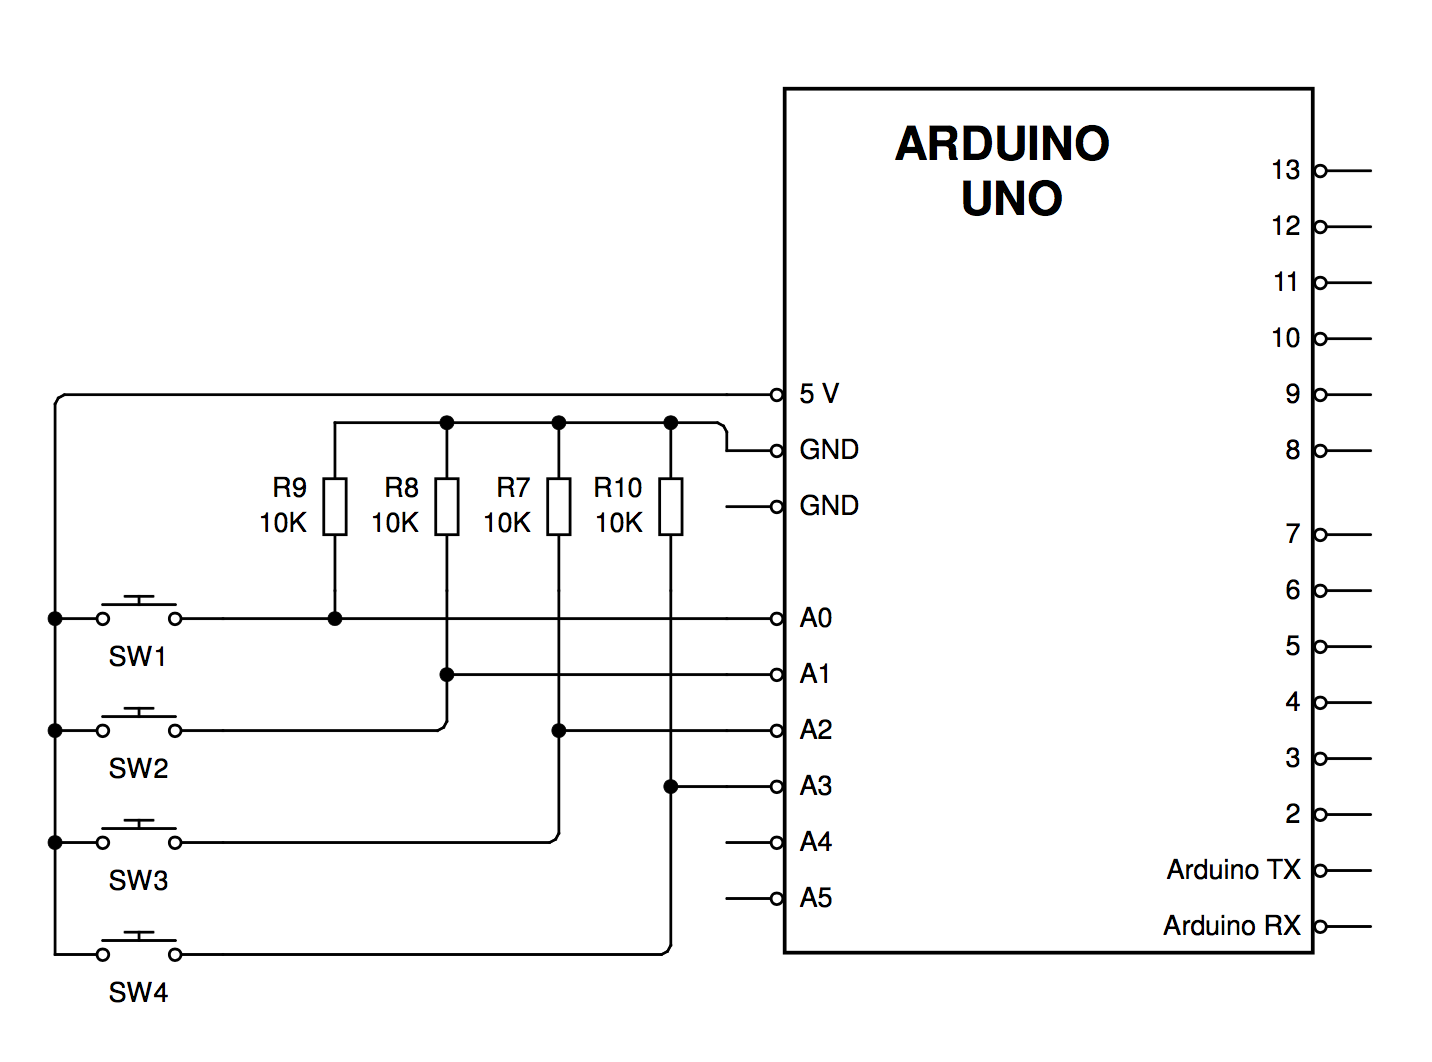
\includegraphics[width=13cm]{figures/CIRCUITS/controllerFinal.png}
	\caption{Et billede af kredsløbet for controller kredsen.}
	\label{kreds:controller}
\end{figure}

\subsection{Komponenter}
I kontrolleren bliver der kun brugt simple fysiske switches, modstande og en Arduino. Se afsnit \ref{sub:arduino} for beskrivelse af Arduino.


\subsection{Teori}
For at undgå en kortslutning bliver der sat en modstand imellem den ene switch side og ground. På den anden side a switchen er der $\SI{5}{V}$.
%\subsection{Beregninger}

%\subsection{Test}